\subsection{Determinação do Momento de Inércia de um disco}

Uma das montagens experimentais que utilizaremos nessa prática é a do Disco de Maxwell. Ela consiste num disco que está preso a um eixo e que possui dois fios de barbante amarrados nas extremidades. Isso permite que ele seja solto de uma altura qualquer e acelere para baixo ganhando energia cinética de translação e rotação, possibilitando fazer uma análise quantitativa desses dois fenômenos. 

\begin{figure}[H]
  \centering
  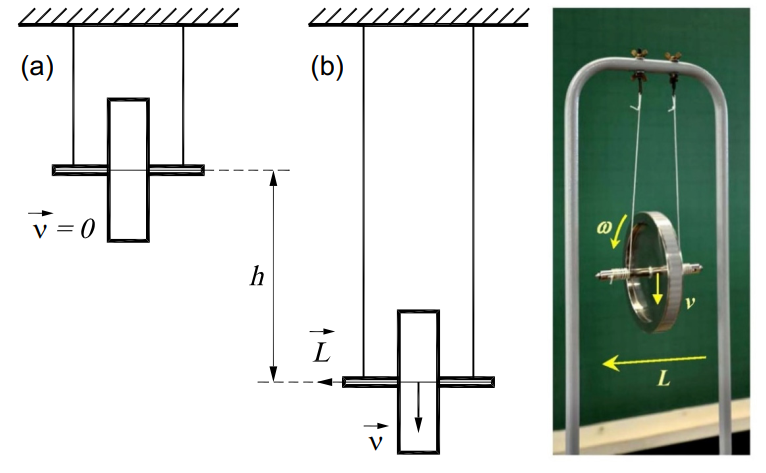
\includegraphics[scale=0.5]{images/setup-maxwell.png}
  \caption{Montagem experimental do Disco de Maxwell}
\end{figure}

Num primeiro momento, desmontaremos o disco e utilizaremos as medidas de cara componente dele para determinar o seu momento de inércia, que será a soma dos momentos de cada componente. Como ele é feito de basicamente um cilindro inteiro (eixo) e 2 cilindros com furo (anel externo + disco), nós sabemos que o momento de inércia total será a soma dos momentos de inércia de cada peça:

\[I_T = I_E + I_A + I_D\]

Com a incerteza sendo a simples soma das incertezas de cada componente:

\[\Delta I_T = \Delta I_E + \Delta I_A + \Delta I_D\]

E o momento de inércia cada um desses componentes pode ser calculado a partir dessas 2 fórmulas para cilindros inteiros (CI) e cilindros com furo (CF):

\[I_{CI} = \frac{1}{2}MR^2\]
\[I_{CF} = \frac{1}{2}M(R^2 + R_1^2)\]

Propagando as incertezas nesses dois casos teremos:

\[\Delta I_{CI} = \frac{1}{2} \left( \Delta M \cdot R^2 + 2 \cdot R \cdot \Delta R \cdot M \right)\]
\[\Delta I_{CF} = \frac{1}{2} 
    \left[ 
        \Delta M \cdot (R^2 + R_1^2) + 
        \left( 2 \cdot R \cdot \Delta R + 2 \cdot R_1 \cdot \Delta R_1 \right) \cdot M
    \right]
\]

Agora, vamos calcular por meio da queda o momento de inércia do disco. Para isso, primeiro precisaremos determinar uma altura \textit{h} para ser o nosso referencial de energia potencial gravitacional. Podemos utilizar o fio totalmente estendido como o ponto mais baixo, e a partir daí enrolar da forma que desejar.\\

Após escolher tal altura será feito 3 medições do tempo de queda de acordo com o esquema (a) e (b) da figura anterior. Essas medições serão feitas com um cronômetro de precisão. Com 3 valores iniciais e finais para \textit{$t_b$} - tempo para chegar no estado (b) - encontrados, faremos a subtração deles e depois uma média aritmética para achar $\overline{t}_b$, e a sua incerteza pelo desvio padrão dessas medidas:

\[\overline{t}_b = \frac{t_{b1} + t_{b2} + t_{b3}}{3}\]

\[\Delta \overline{t}_b = \sqrt{\frac{\sum_{i=1}^{3} (t_i - \overline{t})^2}{3}}\]

Com $\overline{t}_b$ depois poderemos estimar o valor do momento de inércia \textit{I} do disco em estudo e utilizando a seguintes fórmula que foram deduzidas na apostila do curso e nos vídeos, com \textit{r} sendo o raio de giro, ou seja, o raio do eixo:

\[I = \left( \frac{g \overline{t}_b^2}{2h} - 1 \right) mr_e^2\]

E a incerteza \textit{$\Delta$I} dessa medida será dada por:

\[\Delta I = \Delta P \cdot Q + \Delta Q \cdot P\]

Onde \textit{$\Delta$P} é a propagação do que está dentro dos parênteses, e \textit{$\Delta$Q} o termo do lado de fora.

\[
    \Delta P = \frac{g}{2} 
    \left( 
        \frac
        {\overline{t}_b^2 \cdot \Delta H + 2 \cdot \overline{t}_b \cdot \Delta \overline{t}_b \cdot h}
        {h^2} 
    \right)
\]
\[\Delta Q = 2mr \Delta r + \Delta m r^2\]
